\documentclass{article}
\usepackage{a4wide}
\usepackage{graphicx}

\title{Design principles for standing desk computer support}
\author{Cedric Pradalier}


\begin{document}
\maketitle

\section{Principle}
\begin{center}
    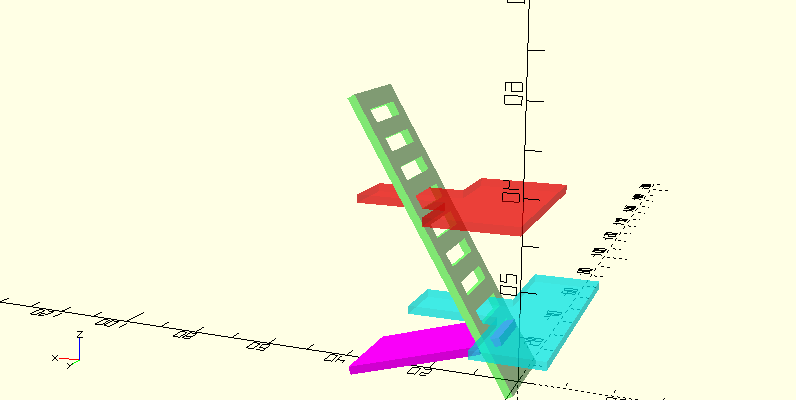
\includegraphics[width=0.7\columnwidth]{../cad/SupportAssisDebout.png}
\end{center}
The core design parameters are the angle $\alpha$ of the ladder, and the thickness $T$ of the wood.

\section{Width of the support tablet}
\begin{center}
    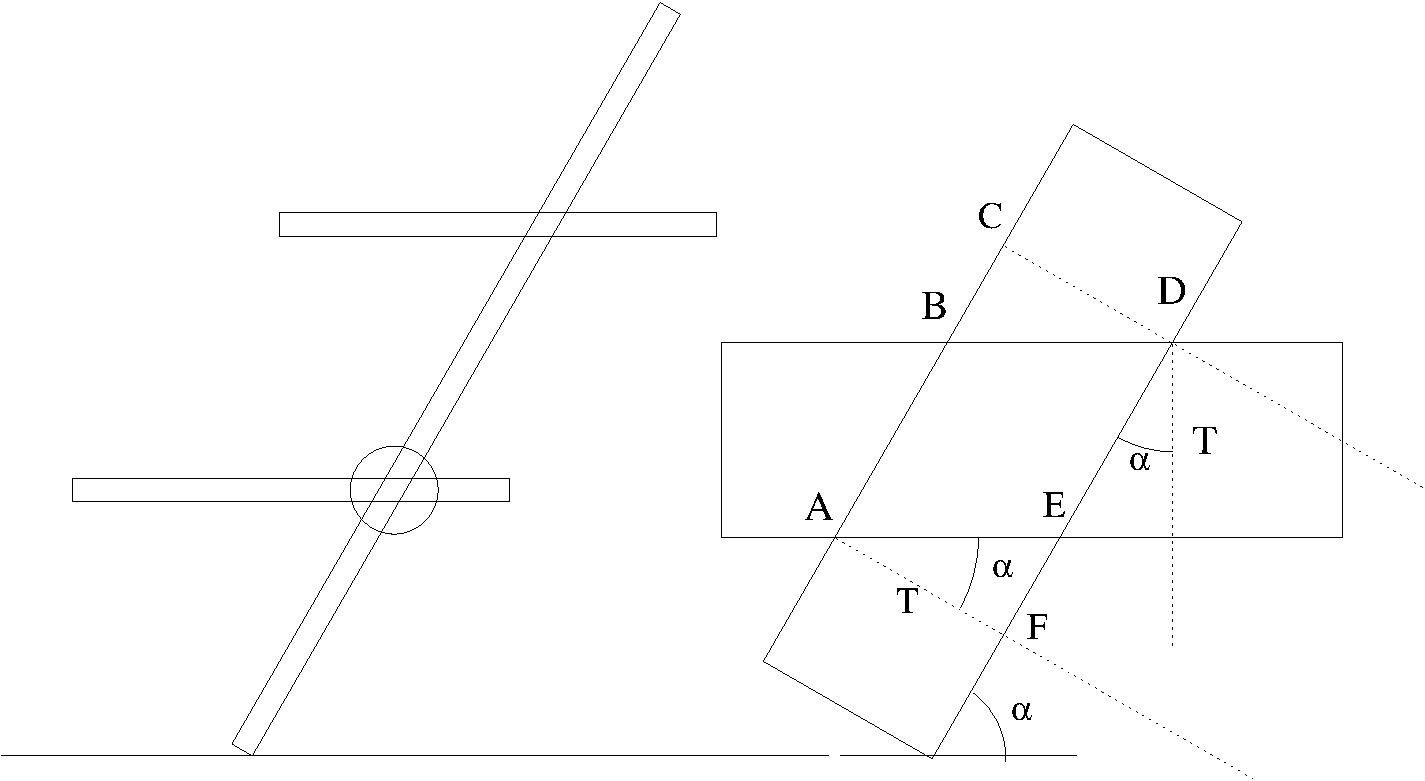
\includegraphics[width=0.7\columnwidth]{slot1.pdf}
\end{center}
The support tablet needs to be horizontal, which happens if the insertion slot defined by the polygon ABCDEF has the right width.

If the tablet is horizontal, we have
$$DE = \frac{T}{\cos\alpha}$$
Which means that:
$$EF = T \tan\alpha$$
So
\begin{equation}
    \label{eq:tablet-slot}
    DF = T\left(\frac{1}{\cos \alpha} + \frac{\sin \alpha}{\cos\alpha}\right) = 
    T \left(\frac{1 + \sin\alpha}{\cos \alpha}\right)
\end{equation}

\section{Design of the support leg}
\begin{center}
    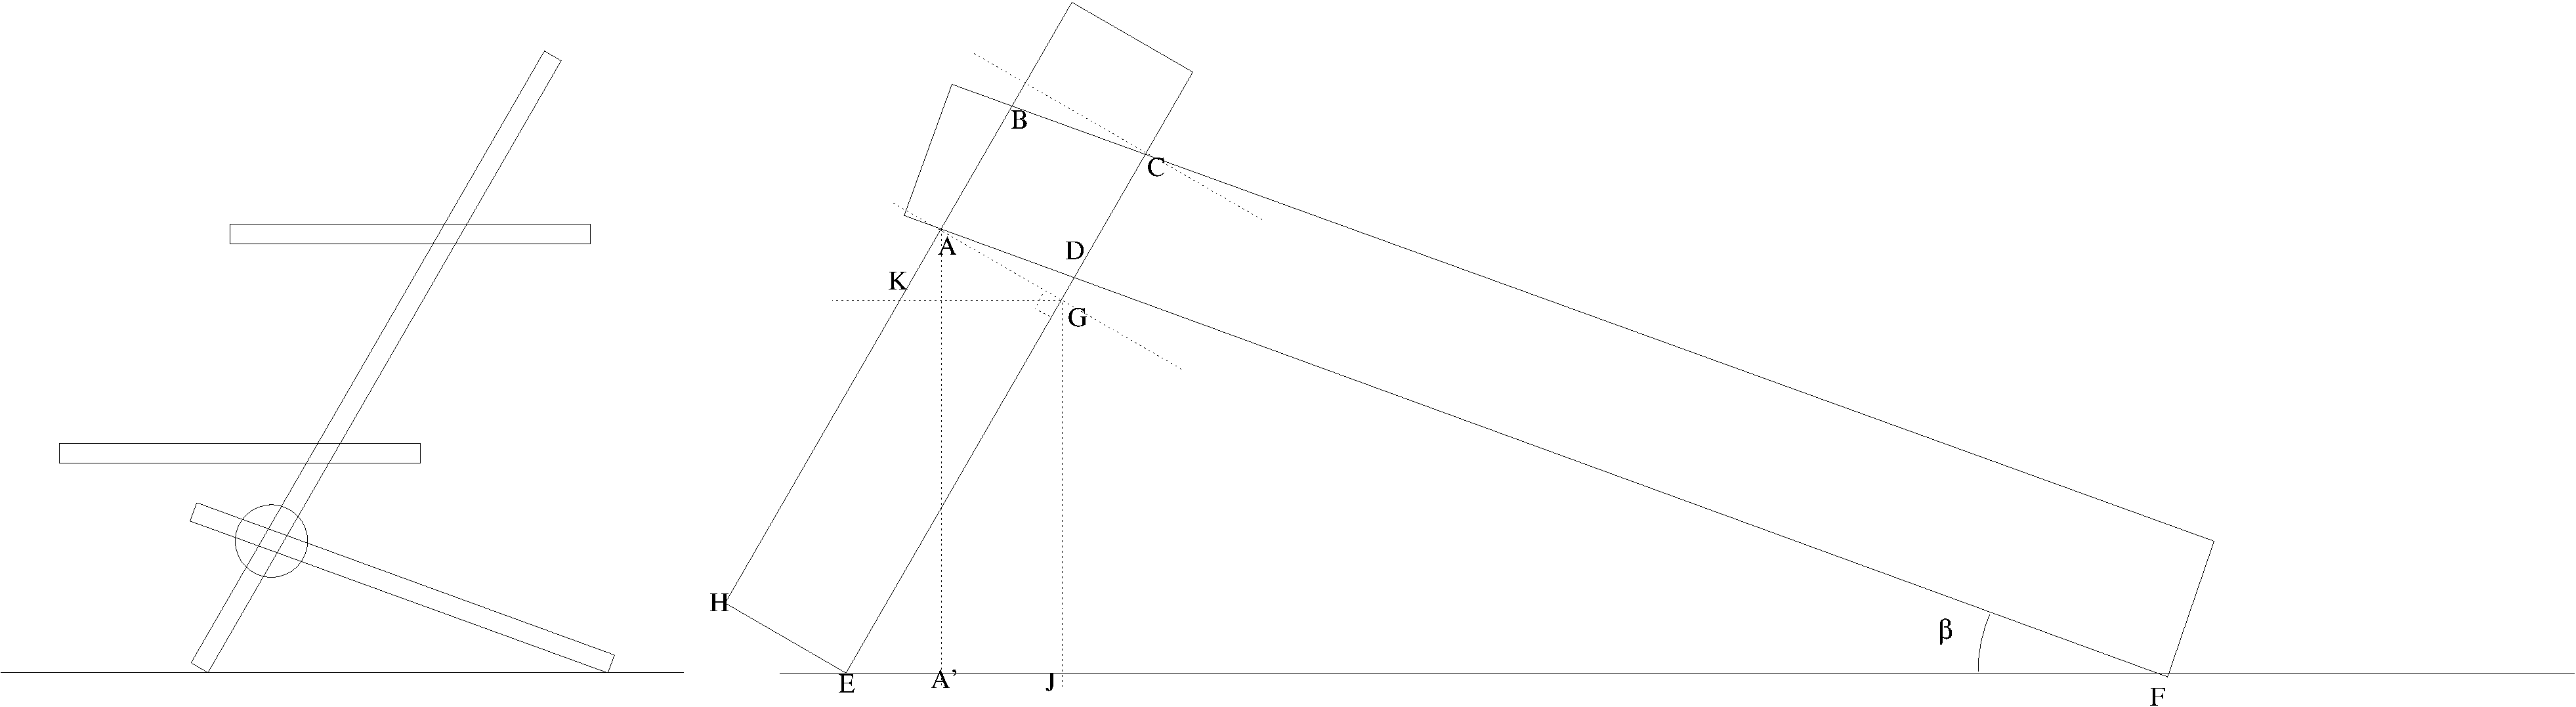
\includegraphics[width=0.99\columnwidth]{slot2.pdf}
\end{center}
Let us first assume that the length of the ladder is $L$. For stability, we assume that $EF = L \sin\alpha$. We now define $p_{leg} = HA$, which is a fourth design parameter.

In order to compute the angle $\beta$, we use the fact that:
$$
\tan \beta = \frac{AA'}{A'F}
$$
We start with $AA' = JG + KA$:
$$
JG = A'G \cos \alpha = p_{leg} \cos \alpha
$$
and 
$$
KA = T \sin \alpha
$$
Then $A'F = EF - (EJ - JA')$:
$$
EJ=p_{leg} \sin \alpha
$$
and 
$$
JA' = GK = T \cos\alpha
$$
Finally:
$$
\beta = \arctan \frac{p_{leg} \cos \alpha + T \sin \alpha}{L\sin\alpha - (p_{leg} \sin \alpha - T \cos \alpha)}
$$
Knowing $\alpha$ and $\beta$, we have:
\begin{equation}
    \label{eq:leg-slot}
    GC =  T \left(\frac{1 + \sin\left(\alpha-\beta\right)}{\cos\left(\alpha-\beta\right)}\right)
\end{equation}
Same formula as eq.~\ref{eq:tablet-slot}. $\alpha-\beta=0$ corresponds to a leg orthogonal to the ladder. 

\section{Insert length}
\begin{center}
    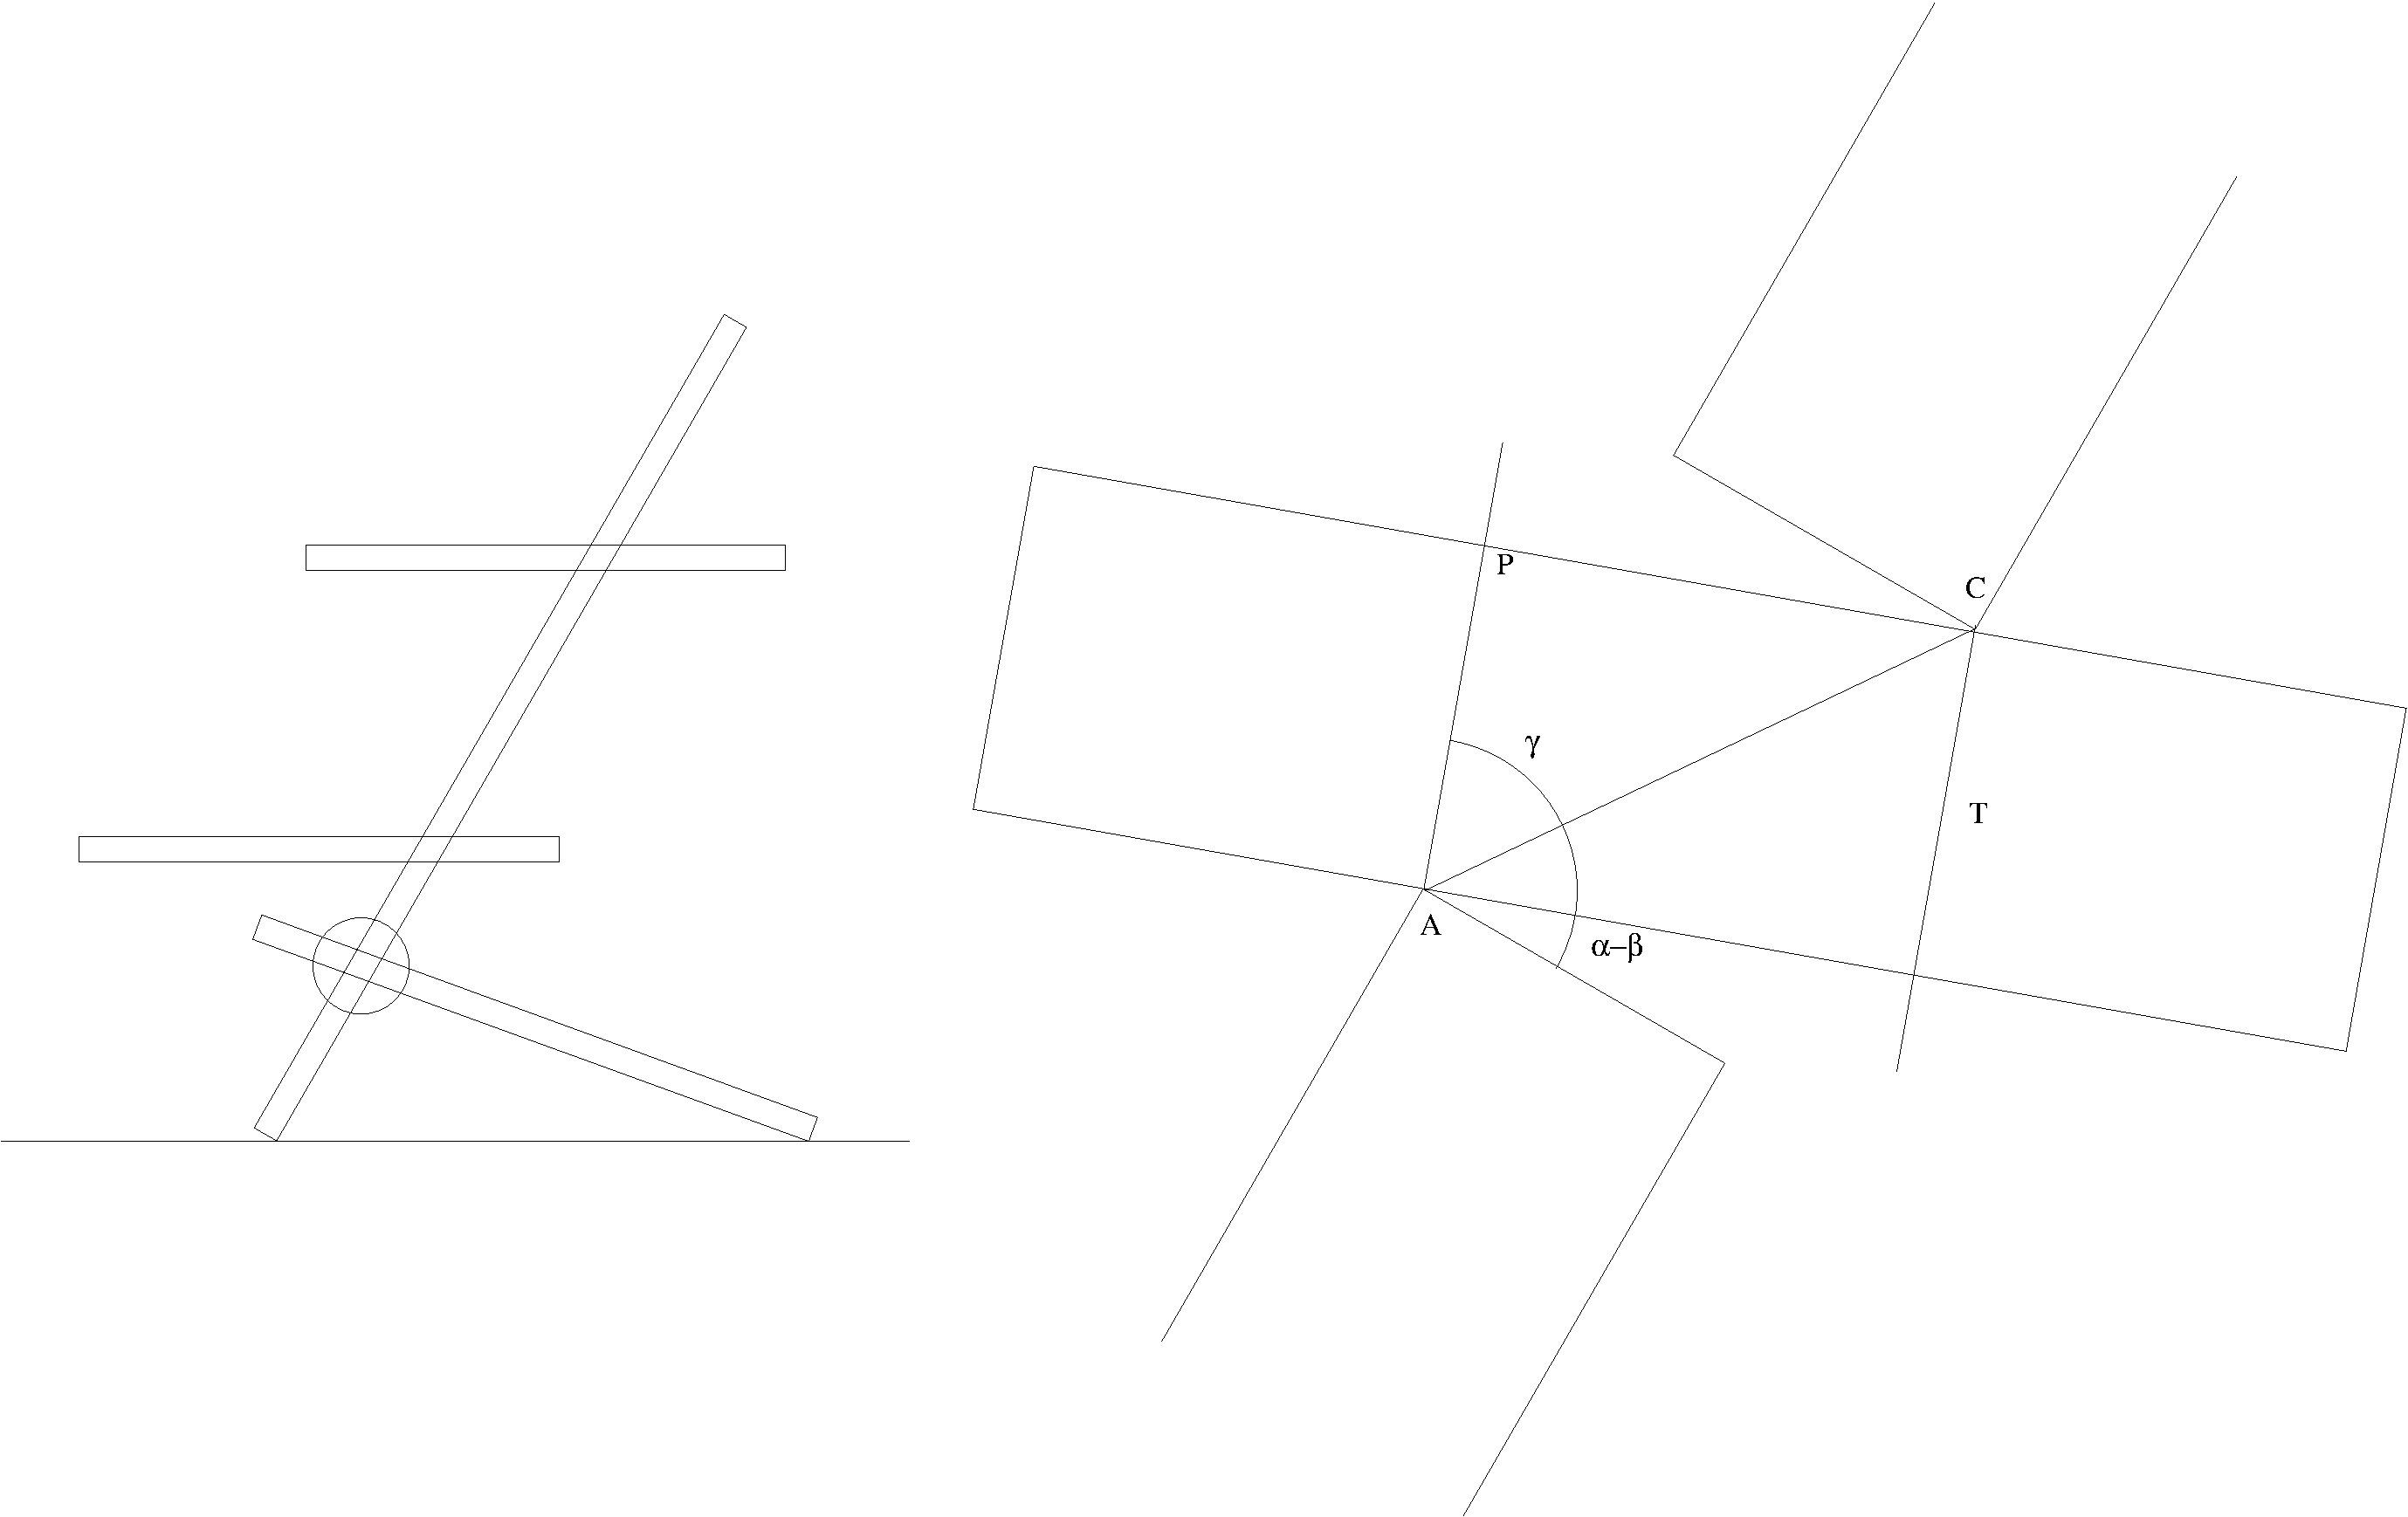
\includegraphics[width=0.99\columnwidth]{slot3.pdf}
\end{center}
The final point is compute to minimal length of the part of the leg inserted into the ladder. The leg will be inserted until the stopper is on C. At this time, the leg still needs to be in contact in A.
We have:
$$
AC = \textrm{hypot}(T,GC)
$$
Also
$$
\sin \gamma = \frac{T}{AC}
$$
Hence:
\begin{equation}
\label{eq:insert}
PC = AC \cos \gamma
\end{equation}
gives us the minimal length of the insert section. 

This also gives us the length $L_{leg}$ of the part of the leg {\bf not} inserted in the ladder:
\begin{equation}
    \label{eq:leglength}
    L_{leg} = \frac{AA'}{\sin\beta} - PC = \frac{p_{leg}\cos\alpha + T \sin \alpha}{\sin \beta} - AC\cos\gamma
\end{equation}

\section{Design example}

The final design, for an angle $\alpha$ of 60 degrees, wood thickness of $T$  of 18mm, $p_{leg}$ of 100mm  is shown here:
\begin{center}
    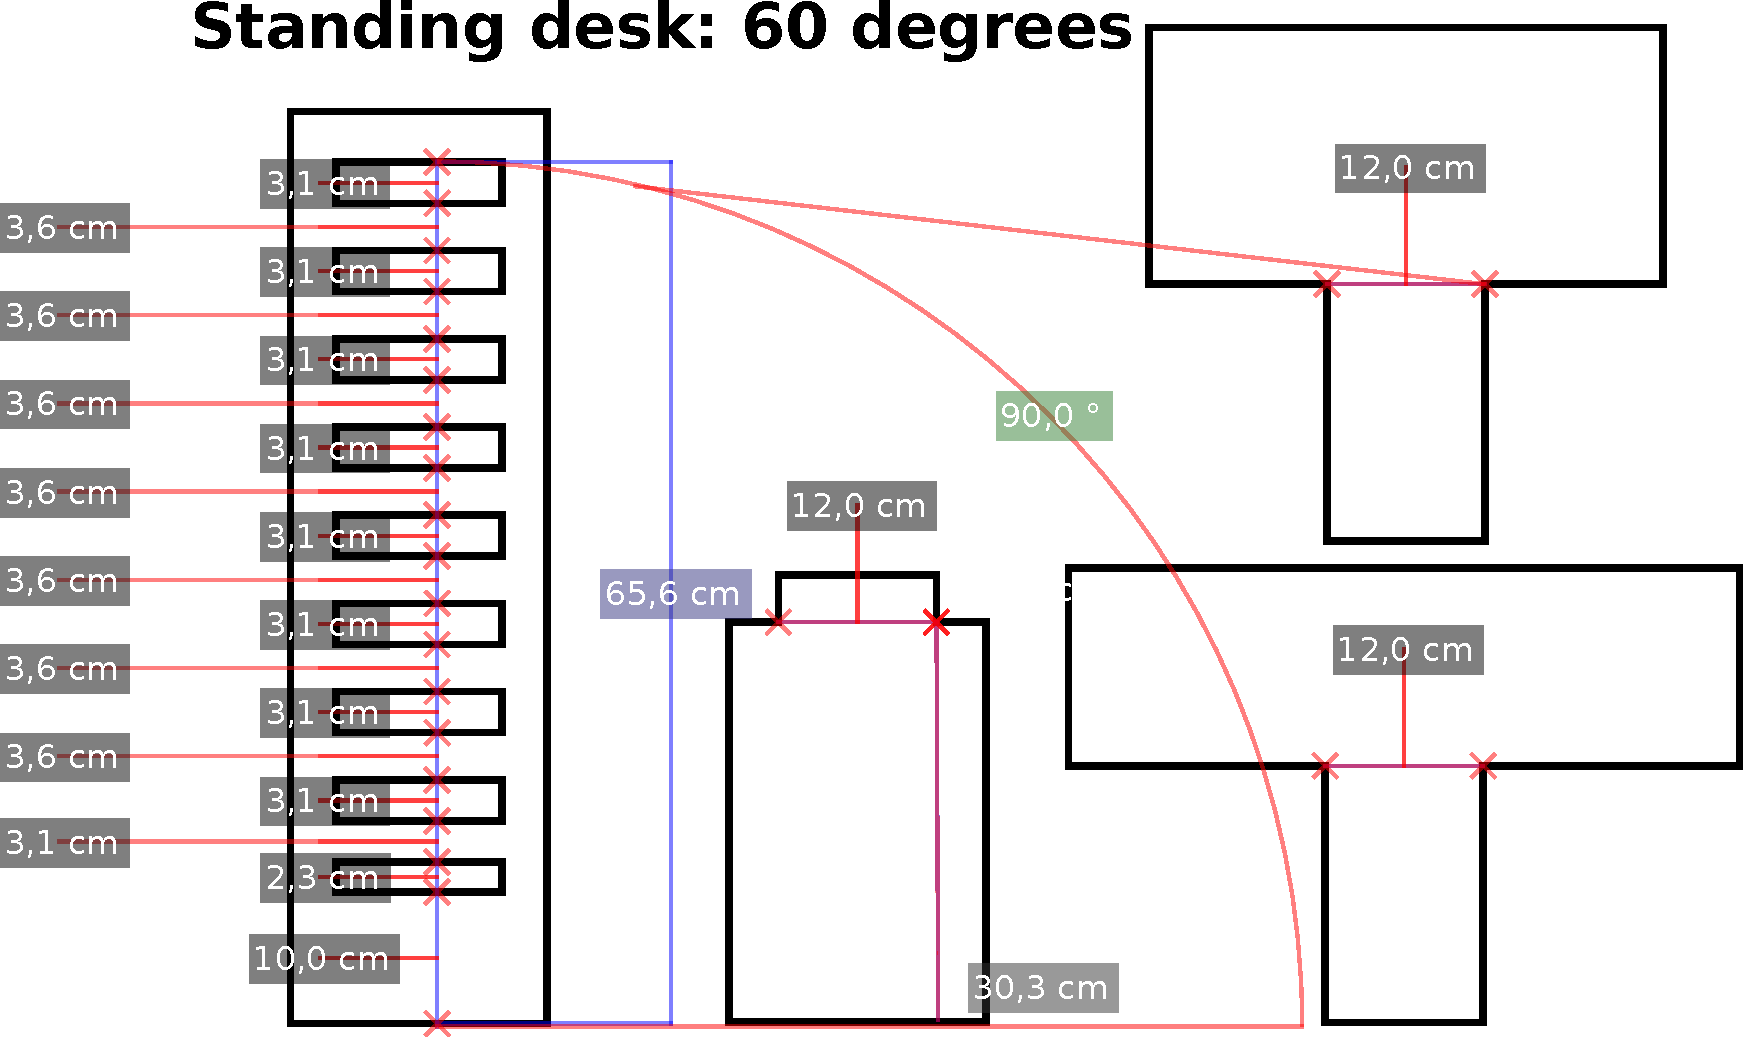
\includegraphics[width=\columnwidth]{../cad/SupportAssisDeboutCut.pdf}
\end{center}
The resulting assembly is shown here:
\begin{center}
    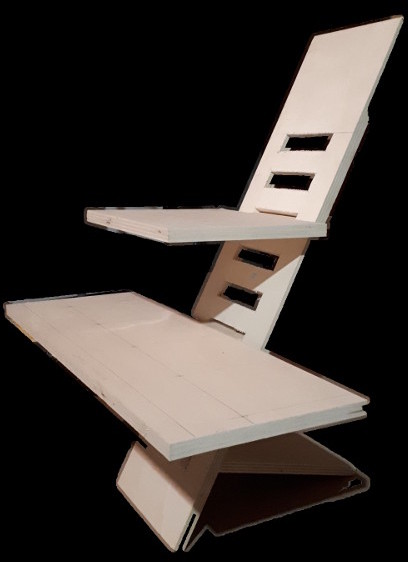
\includegraphics[width=0.4\columnwidth]{../pics/IMG_20210303_231314.jpg}
    \hfill
    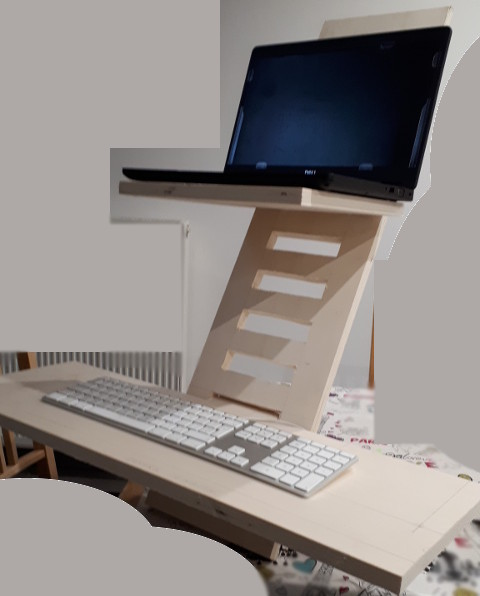
\includegraphics[width=0.4\columnwidth]{../pics/IMG_20210303_232329.jpg}
\end{center}

\end{document}
